\section{Example of usage}\label{sec:examples}

\subsection{Setting up spacecraft ADCS architecture in SCARS}

\subsubsection{Basic made up spacecraft}

\subsubsection{PW-Sat2}
    Magnetorquers

    Two modes of control: Detumbling Control Mode; Sun Pointing Mode
    % https://pw-sat.pl/wp-content/uploads/2014/07/PW-Sat2-C-01.00-ADCS-CDR.pdf

    \paragraph*{Detumbling}\hspace{0pt} \\
        Detumbling maneuver is performed after deployment of the spacecraft from a carrier rocket. As the satellites are separated from the deployment mechanism, they are burdened by non-zero initial angular rates. To counteract that and stabilize a satellite PW-Sat2 is equipped with a set of two perpendicular magnetorquer rods and one air core, in total one coil acting along each of satellite's body axis. The most important parameters used by \ac{scars} model of PW-Sat2 are listed in Table \ref{table:pwsat2magne}.\cite{pwsat2adcs} Exact values are taken directly from the datasheet of \ac{imqt}.\cite{imqt-datasheet}

        \begin{center}    
            \begin{tabular}{l l}
                \textbf{Parameter} & \textbf{Value} \\ \hline
                Nominal magnetic dipole & $0.2 Am^2$ \\
                Maximum actuation envelope error & $3\mu T$ \\
                Power consumption during actuation & $1.2W$ \\
                Mass & 196g
            \end{tabular}
        \end{center}\label{table:pwsat2magne}


    \paragraph*{Deorbitation with drag sail}\hspace{0pt} \\
        One of the main objectives of PW-Sat2 mission was to deploy and test the effectiveness of it's drag sail in deorbitation maneuver. The sail was  $2$x$2m$ square made from aluminized polyester boPET film.\cite{pwsat2dt}
        
        In this example, \ac{scars} toolbox was tested against data points derived from NORAD measurements. The simulation was run in two cases: only with drag sail set up and with drag sail and magnetorquers on to keep sail's plane perpendicular to spacecraft's orbit tangent vector.
         
        \begin{figure}[H]
            \centering
            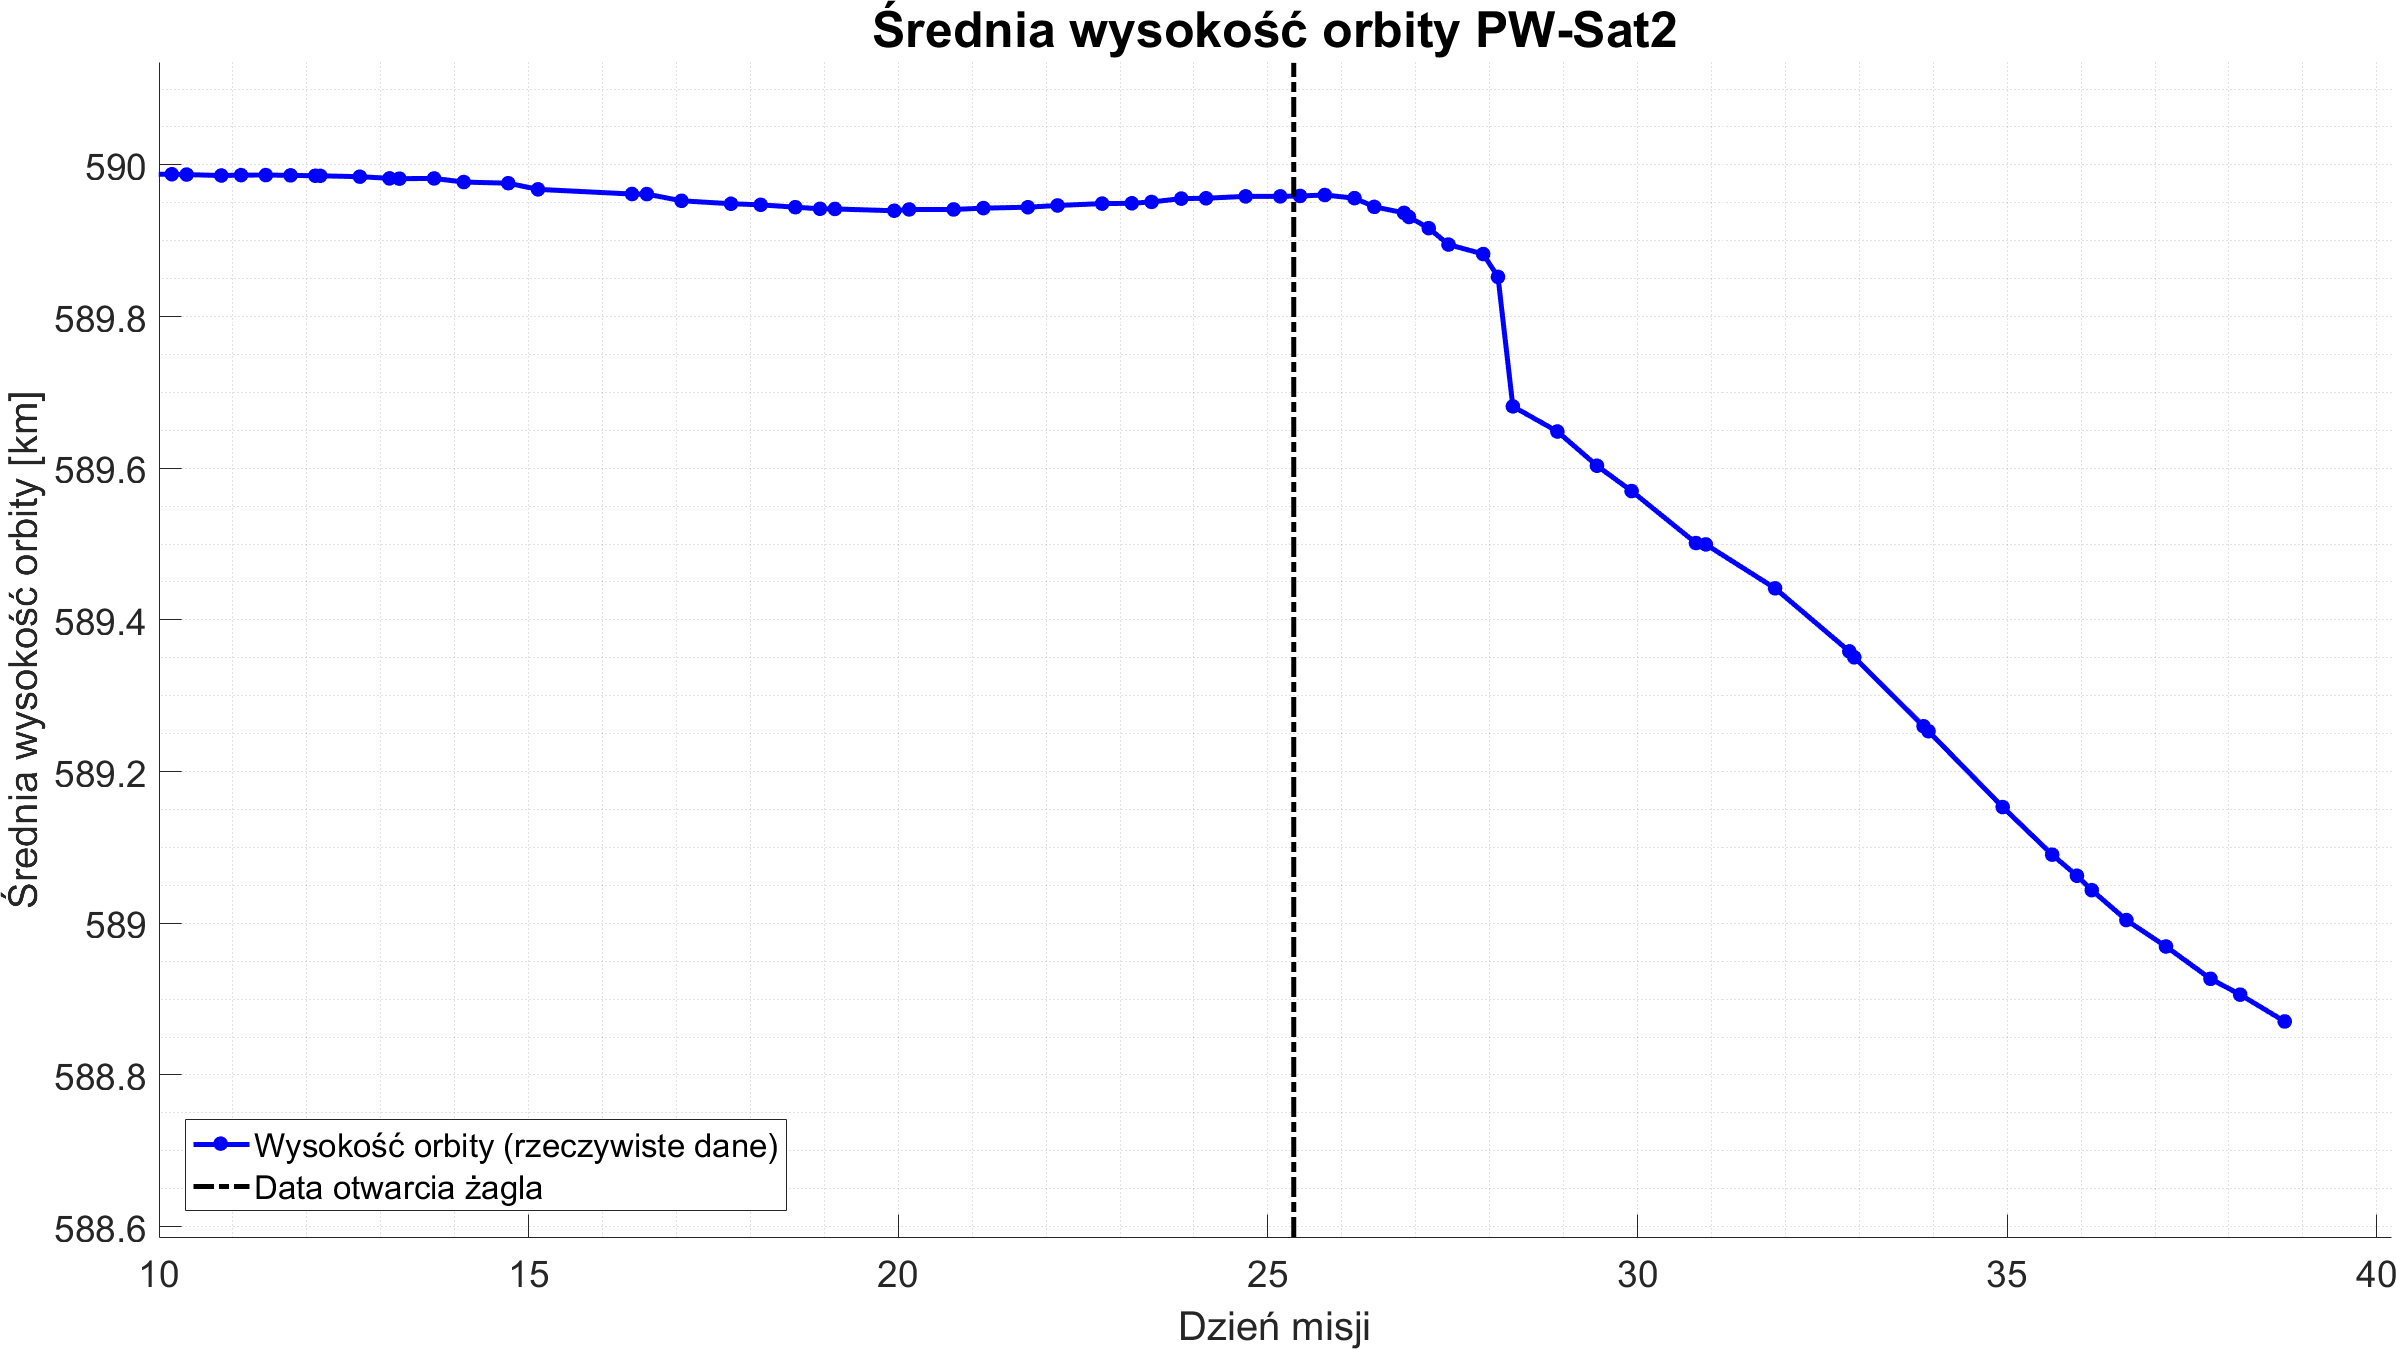
\includegraphics[width=1\textwidth]{4-examples/pw-sat-deorbit.png}
            \caption{Average altitude of PW-Sat2 satellite as taken from NORAD measurements. On X axis there is mission time in days, on Y axis there is average altitude in km.}
            \label{fig:pw-sat-deorbit}
        \end{figure}
         
        \begin{figure}[H]
            \centering
            \includegraphics[width=1\textwidth, height=160px]{example-image-a}
            \caption{Results from \ac{scars} simulation, with only drag sail included}
            \label{fig:scars-deorbit}
        \end{figure}
         
        \begin{figure}[H]
            \centering
            \includegraphics[width=1\textwidth, height=160px]{example-image-b}
            \caption{Results from \ac{scars} simulation, with magnetorquer-driven attitude correction}
            \label{fig:scars-deorbit}
        \end{figure}


    % \subsubsection{PROBA-1}
    % https://directory.eoportal.org/web/eoportal/satellite-missions/p/proba-1#spacecraft


    \subsubsection{Sentinel-2} 
    
    Sentinel-2 is a European polar satellite mission carried out by \ac{esa} as a part of Copernicus Programme. It consists of constellation of twin polar orbit satellites, Sentinel-2A and Sentinel-2B and it's aim is to deliver Earth observation data to broad public, providing wide range of services such as natural emergency management, agricultural monitoring or water classification. \cite{sentinelreference_description}

    As per document describing Sentinel-2 \ac{adcs} subsystem, the satellites operate on a sun-synchronous oribt, with $786km$ mean altitude and $10:30$ local time of descending node. They maintain Earth-oriented attitude in all operational modes. The required pointing performance is moderate, but the main design driver is the need for precise geo-location of the images. \cite{sentinelreference_adcs}

    The actuators on board of Sentinel-2 and simulated with \ac{scars} toolbox for demonstration purposes are decribed in Table \ref{table:sentinel-adcs}.

    % Gyro: https://spaceequipment.airbusdefenceandspace.com/avionics/fiber-optic-gyroscopes/astrix-200/
    % Thrusters: https://www.yumpu.com/en/document/read/10860453/1-n-monopropellant-thruster-astrium-st-eads
    % Magnetometer: http://www.zarmtec.uni-bremen.de/products/magnetometer/
        
    \begin{center}    
        \begin{tabular}{ c l l l l }
            \textbf{No.} & \textbf{Uni}t & \textbf{Type} & \textbf{Supplier} & \textbf{Name} \\ \hline
            3 & MAG & 3-axis fluxgate magnetometer & ZARM Technik & FGM-A-75 \\
            2 & GPRS & 2 band GPS receiver & RUAG & - \\
            3 & STR  & Active pixel sensor star tracker & Jena Optronik & Astro APS \\
            4 & IMU & High performance fibre optical gyro & Astrium & ASTRIX 200 \\
            3 & MTQ & $140 Am^2$ magnetic torquer & ZARM Technik & MT140-2\\
            4 & RW & $18 Nms$ reaction wheel & Honeywell & HR12 \\
            8 & THR & $1N$ monopropellant thruster & EADS ST &CHTIN-6
        \end{tabular}
    \end{center}\label{table:sentinel-adcs}

\subsection{Examples of tests possible with SCARS}

\subsubsection{Control system robusntess analisys}

\subsubsection{Long term simulation}

\subsubsection{Contingency scenarios}
